% gCOVguide.tex
% v4.0 released February 2015

\documentclass{gCOV2e}

\usepackage{epstopdf}% To incorporate .eps illustrations using PDFLaTeX, etc.
\usepackage{subfigure}% Support for small, `sub' figures and tables

\theoremstyle{plain}% Theorem-like structures
\newtheorem{theorem}{Theorem}[section]
\newtheorem{corollary}[theorem]{Corollary}
\newtheorem{lemma}[theorem]{Lemma}
\newtheorem{proposition}[theorem]{Proposition}

\theoremstyle{definition}
\newtheorem{definition}[theorem]{Definition}
\newtheorem{example}[theorem]{Example}

\theoremstyle{remark}
\newtheorem{remark}[theorem]{Remark}

\newcommand{\mcO}{\mathcal{O}} % Big O
\newcommand{\iu}{{i\mkern1mu}} % imaginary unit
\newcommand{\eexp}[1]{e^{#1}}  % convenient exponent

\renewcommand{\Re}{\operatorname{Re}} % default Re/Im is weird
\renewcommand{\Im}{\operatorname{Im}}

% \DeclarePairedDelimiter\abs{\lvert}{\rvert}%
% \DeclarePairedDelimiter\norm{\lVert}{\rVert}%

\newcommand\abs[1]{\left|#1\right|}
\DeclareMathOperator\asin{asin}
\DeclareMathOperator\atanh{atanh}
\begin{document}

%\jvol{00} \jnum{00} \jyear{2015} \jmonth{February}

\articletype{GUIDE}

\title{\textit{Complex Variables and Elliptic Equations} \LaTeX\ guide for authors (Style 2 + NLM reference style)}

\author{
\name{A.N. Author\textsuperscript{a}$^{\ast}$\thanks{$^\ast$Corresponding author. Email: latex.helpdesk@tandf.co.uk}
and I.T. Consultant\textsuperscript{b}}
\affil{\textsuperscript{a}Taylor \& Francis, 4 Park Square, Milton Park, Abingdon, UK;
\textsuperscript{b}Institut f\"{u}r Informatik, Albert-Ludwigs-Universit\"{a}t, Freiburg, Germany}
\received{v4.0 released February 2015}
}

\maketitle

\begin{abstract}
This guide is for authors who are preparing papers for \textit{Complex Variables and Elliptic Equations} (\textit{gCOV})
using the \LaTeX\ document preparation system and the class file \texttt{gCOV2e.cls},
which is available via the journal's home page on the Taylor \& Francis website.
\end{abstract}

\begin{keywords}
submission instructions; source file coding; environments; references citation; fonts; numbering
\textbf{(Please provide three to six keywords taken from terms used in your manuscript)}
\end{keywords}

\begin{classcode}F1.1; F4.3 \textbf{(... for example; authors are encouraged to provide two to six 2010 Mathematics Subject Classification codes)}\end{classcode}


{\abstractfont\centerline{\bfseries Index to information contained in this guide}\vspace{12pt}
\hbox to \textwidth{\hsize\textwidth\vbox{\hsize17pc
\hspace*{-12pt} {1.}    Introduction\\
\hspace*{7pt} {1.1.}  The \textit{gCOV} document class\\
\hspace*{7pt} {1.2.}  Submission of \LaTeX\ articles\\
\hspace*{24pt}        to the journal\\
{2.}    Using the \textit{gCOV} class file\\
{3.}    Additional features\\
\hspace*{10pt}{3.1.}  Title, authors' names, abstract\\
\hspace*{24pt}        and keywords\\
\hspace*{10pt}{3.2.}  Additional footnotes to the\\
\hspace*{24pt}        title or authors' names\\
\hspace*{10pt}{3.3.}  Lists\\
{4.}    Some guidelines for using\\
\hspace*{6pt}        standard features\\
\hspace*{10pt}{4.1.}  Sections\\
\hspace*{10pt}{4.2.}  Illustrations (figures)\\
\hspace*{10pt}{4.3.}  Tables\\
\hspace*{10pt}{4.4.}  Landscape pages\\
\hspace*{10pt}{4.5.}   Theorem-like environments\\
\noindent \hspace*{7pt} {4.6.}   Typesetting mathematics\\
\hspace*{24pt} {4.6.1.}  Displayed mathematics\\
\hspace*{24pt} {4.6.2.}  Bold math italic symbols\\
\hspace*{24pt} {4.6.3.}  Bold Greek\\
\hspace*{24pt} {4.6.4.}  Upright Greek characters \\
\hspace*{47pt}            and the upright partial \\
\hspace*{47pt}            derivative sign }
\hspace{-24pt}\vbox{\noindent\hsize17pc
\hspace*{7pt} {4.7.}   Acknowledgements \\
\hspace*{7pt} {4.8.}   Disclosure \\
\hspace*{7pt} {4.9.}   Funding \\
\hspace*{7pt} {4.10.}   Notes \\
\hspace*{7pt} {4.11.}   Supplemental material \\
\hspace*{7pt} {4.12.}   References \\
\hspace*{24pt} {4.12.1.}  References cited in the \\
\hspace*{52pt}            text\\
\hspace*{24pt} {4.12.2.}  The list of references\\
\hspace*{7pt} {4.13.}   Appendices \\
{5.}    Example of a section heading \\*
\hspace*{6pt}   including {\fontencoding{T1}\scshape{small caps}}, \textit{italic}, \\
\hspace*{6pt}   and bold Greek such as ${\bm\kappa}$ \\
{6.}    \textit{gCOV} journal style \\
\hspace*{10pt}{6.1.}   Hyphens, en rules, em rules \\ \hspace*{27pt}and minus signs\\
\hspace*{10pt}{6.2.}   References \\
\hspace*{10pt}{6.3.}   Maths fonts\\
{7.}    Troubleshooting\\
{8.}    Fixes for coding problems\\
{9.}    Obtaining the \texttt{gCOV2e} class file\\
\hspace*{10pt}{9.1}  Via the Taylor \& Francis \\
\hspace*{24pt}       website\\
\hspace*{10pt}{9.2}  Via e-mail\\}}}


\section{Introduction}

????? 

% In order to assist authors in the process of preparing a manuscript for \textit{Complex Variables and Elliptic Equations} (\textit{gCOV}), the journal's layout style has been implemented as a \LaTeXe\ class file based on the \texttt{article} document class. A \textsc{Bib}\TeX\ style file is also provided to assist with the formatting of your references in a style appropriate to that of the journal.

% Commands that differ from or are provided in addition to the standard \LaTeXe\ interface are explained in this guide. The guide alone is not intended as a substitute for an appropriate \LaTeXe\ manual.

% The \texttt{gCOVguide.tex} file can also be used as a template for composing an article for submission by cutting, pasting, inserting and
% deleting text as appropriate, using the \LaTeX\ environments provided (e.g. \verb"\begin{equation}", \verb"\begin{enumerate}").

% \textbf{Please note that the index following the abstract in this guide is provided for information only. An index is not required in submitted papers.}

\section{Definitions and notation}

\subsection{Notation}

\begin{itemize}
\item $\mathbb{C}$: complex plane, $\mathbb{C} = \{ x + \iu y \mid x, y \in \mathbb{R} \}$ 
\item $\mathbb{H}$: upper complex half-plane, $\mathbb{H} = \{ x + \iu y \mid y > 0, x, y \in \mathbb{R} \}$
\item $\mathbb{D}$: unit disk, $\mathbb{D} = \{ z \mid \abs{z} < 1 \}$
\item $\mathbb{T}$: unit circle, $\mathbb{T} = \partial \mathbb{D} =  \{z \mid \abs{z} = 1 \}$
\item $z$ denotes a complex argument on complex plane $\mathbb{C}$
\item $\zeta$ denotes a complex argument on unit disk $\mathbb{D}$
\end{itemize}

\subsection{Cayley transform}

Cayley transform maps $\mathbb{H}$ to $\mathbb{D}$:
\begin{equation}\label{eq:cayley}
W(z) = \frac{z - \iu}{z + \iu}
\end{equation}
, whereas inverse Cayley transform maps $\mathbb{D}$ to $\mathbb{H}$:
\begin{equation}\label{eq:cayley_inverse}
w(\zeta) = \iu \frac{1 + \zeta}{1 - \zeta}
\end{equation}

One notable property of the Cayley transform is that it injectively maps $\mathbb{R}$ into unit circle $\mathbb{T}$.

Another important property we are going to use is that Cayley transform preserves circles. In particular, a circle with radius $r < 1$ centered in zero, under inverse Cayley transform maps into a circle with center $\iu C(r)$ and radius $R(r)$, where:

\begin{equation}\label{eq:c_and_r}
\begin{aligned}
   C(r) &= \Im \frac{w(r) + w(-r)}{2} = \frac{1 + r^2}{1 - r^2}
\\ R(r) &= \Im \frac{w(r) - w(-r)}{2} = \frac{2 r}{1 - r^2}
\end{aligned}
\end{equation}

From these formulas it's easy to see that if we limit $r$ to $1$, $R(r)$ goes to infinity and $C(r)$ converges to $R(r)$.

Also, we'll note two useful facts:
\begin{itemize}
\item $C(r) - R(r) > 0$
\item $C(r) - R(r) = \frac{1 - r}{1 + r} < \frac{1}{R(r)} = \frac{1 - r^2}{2 r}$, which means that $C - R$ is $\mcO(\frac{1}{R})$
\end{itemize}

\subsection{S-matrix}\label{sec:smatrix}
Consider a localized one dimensional potential barrier or resonator. We assume that the system evolves under the stationary Schrodinger's equation. Since we are only interested in the mathematical scattering problem and scattering state solutions, we set Plank's constant to $1$.

From the left and right we subject in to beams of quantum particles with the wavevector $k$, which will be a scalar in 1D case. Outside the potential barrier the particles behave as plane waves:

\begin{equation}\label{eq:wlwl}
\begin{aligned}
   \psi_L(x) &= A \eexp{\iu k x} + B \eexp{-\iu k x}
\\ \psi_R(x) &= C \eexp{\iu k x} + D \eexp{-\iu k x}
\end{aligned}
\end{equation}

S-matrix, or scattering matrix relates the final and initial states of the system:
\begin{equation}\label{eq:smatrix}
\begin{pmatrix} B \\ C \end{pmatrix} = S \begin{pmatrix} A \\ D \end{pmatrix}
\end{equation}
, and defines scattering properties of a potential barrier.

\section{Convergence criterion}
There is a connection between the S-matrix and the completeness of the resonant states for a scattering problem:

TODO something about dissipating operator

\begin{theorem}[{\cite[p. 95]{nikol2012treatise}}, {\cite[p. 99]{nikol2012treatise}}]
The following statements are equivalent:
\begin{itemize}
\item the dissipating operator $Z$ is complete
\item
\begin{equation}\label{eq:blaschke}
\lim\limits_{r = 1} \int\limits_{\mathbb{T}} \log \abs{\det S(r \zeta)} d m(\zeta) = 0
\end{equation}
\end{itemize}
\end{theorem}

We will use the criterion (\ref{eq:blaschke}) to analyse the completeness of the system of resonant states. In the space of the unit disk it looks like:
\begin{equation}\label{eq:crit_cayley}
\lim\limits_{r = 1} \int\limits_{\abs{\zeta} = r} \log \abs{\det S(\zeta)} d \zeta = 0
\end{equation}

Since S-matrix is naturally defined on the complex plance, it makes sense to use the upper complex plane for the analysis of completeness. We change the variable in (\ref{eq:crit_cayley}), applying Cayley transform to the integral, which results in:

\begin{equation}\label{eq:crit}
\lim\limits_{r \to 1} \int\limits_{C_r} \ln \abs{\det S(k)} \frac{2 \iu}{(k + i)^2} dk = 0
\end{equation}
, where $C_r$ is an image of $\abs{\zeta} = r$ under the inverse Cayley transform. It can be parameterised as $C_r = \{R(r) \eexp{\iu t} + \iu C(r) \mid t \in [0, 2 \pi)\}$ (see \ref{eq:c_and_r}). For brevity, define:

\[
s(k) = \abs{\det S(k)}
\]
, and after throwing away constants which are irrelevant for convergence, we get the final form of the criterion, which is convenient for us and will be used afterwards:

\begin{equation}\label{eq:critp}
\lim\limits_{r \to 1} \int\limits_{0}^{2 \pi} \ln s(R(r) \eexp{\iu t} + \iu C(r)) \frac{R}{(R(r) \eexp{\iu t} + \iu C(r) + i)^2} dt = 0
\end{equation}


\section{Description of model}




\section{Proof of completeness of resonant states}

\section{Using the \textit{gCOV} class file}

If the file \texttt{gCOV2e.cls} is not already in the appropriate system directory for \LaTeXe\ files, either
arrange for it to be put there, or simply copy it to your working folder. In order to use the \textit{gCOV} document class, replace the command
\verb"\documentclass{article}" at the beginning of your document with the command \verb"\documentclass{gCOV2e}".

The following document-class options should \emph{not} be used with the \textit{gCOV} class file:
\begin{itemize}
  \item \texttt{10pt}, \texttt{11pt}, \texttt{12pt} -- unavailable;
  \item \texttt{oneside}, \texttt{twoside} -- not necessary, oneside is the default;
  \item \texttt{leqno}, \texttt{titlepage} -- should not be used;
  \item \texttt{onecolumn} -- not necessary as it is the default style.
\end{itemize}
The \texttt{geometry} package and commands associated with it should also not be used to adjust the page dimensions.


\section{Additional features}

\subsection{Title, authors' names, abstract and keywords}

The title should be generated at the beginning of your article using the \verb"\maketitle" command.
In the final version, the author name(s) and affiliation(s) must be followed immediately by \verb"\maketitle" as shown below in order for them to be displayed in your PDF document.
To prepare an anonymous version for peer review, you can put the \verb"\maketitle" between the \verb"\title" and the \verb"\author" in order to conceal the authors' identities from the reviewers.
Next you should include an abstract, which should be enclosed within an \texttt{abstract} environment.
For example, the titles for this guide begin as follows:
\begin{verbatim}
\title{\textit{Complex Variables and Elliptic Equations} \LaTeX\
guide for authors (Style 2 + NLM reference style)}

\author{
\name{A.N. Author\textsuperscript{a}$^{\ast}$\thanks{$^\ast$Corresponding
author. Email: latex.helpdesk@tandf.co.uk}
and I.T. Consultant\textsuperscript{b}}
\affil{\textsuperscript{a}Taylor \& Francis, 4 Park Square, Milton
Park, Abingdon, UK; \textsuperscript{b}Institut f\"{u}r Informatik,
Albert-Ludwigs-Universit\"{a}t, Freiburg, Germany}
\received{v4.0 released February 2015} }

\maketitle

\begin{abstract}
This guide is for authors who are preparing papers for \textit{Complex
Variables and Elliptic Equations} (\textit{gCOV}) using the \LaTeX\
document preparation system and the class file \texttt{gCOV2e.cls},
which is available via the journal's home page on the Taylor \&
Francis website.
\end{abstract}
\end{verbatim}
A list of keywords should follow the abstract, enclosed within a \texttt{keywords} environment, followed by subject classification codes enclosed within a \texttt{classcode} environment.


\subsection{Additional footnotes to the title or authors' names}

The \verb"\thanks" command may be used to produce additional footnotes to the title or authors' names if required.
Footnote symbols for this purpose should be used in the order:
$\dagger$ (coded as \verb"\dagger"), $\ddagger$ (\verb"\ddagger"), $\S$ (\verb"\S"), $\P$ (\verb"\P"), $\|$ (\verb"\|"),\break
$\dagger\dagger$ (\verb"\dagger\dagger"), $\ddagger\ddagger$ (\verb"\ddagger\ddagger"), $\S\S$ (\verb"\S\S"),
$\P\P$ (\verb"\P\P"), $\|\|$ (\verb"\|\|").

Note that any \verb"footnote"s to the main text will automatically be assigned the superscript
 symbols 1, 2, 3, etc. by the class file.\footnote{If preferred, the \texttt{endnotes} package
 may be used to set the notes at the end of your text, before the bibliography.
 The symbols will be changed to match the style of the journal if necessary by the typesetter.}


\subsection{Lists}

The \textit{gCOV} class file provides numbered and unnumbered lists using the \texttt{enumerate} environment and bulleted
lists using the \texttt{itemize} environment.

The enumerated list will number each list item with arabic numerals by default. For example,
\begin{enumerate}
  \item first item
  \item second item
  \item third item
\end{enumerate}
was produced by
\begin{verbatim}
\begin{enumerate}
  \item first item
  \item second item
  \item third item
\end{enumerate}
\end{verbatim}
Alternative numbering styles can be achieved by inserting an optional argument in square brackets to each \verb"item", e.g. \verb"\item[(i)] first item"\, to create a list numbered with roman numerals.

Unnumbered lists can also be produced using the \texttt{enumerate} environment, e.g.
\begin{enumerate}
  \item[] First unnumbered item
  \item[] Second unnumbered item
  \item[] Third unnumbered item
\end{enumerate}
was produced by
\begin{verbatim}
\begin{enumerate}
  \item[] First unnumbered item
  \item[] Second unnumbered item
  \item[] Third unnumbered item
\end{enumerate}
\end{verbatim}

Bulleted lists are provided using the \texttt{itemize} environment. For example,
\begin{itemize}
  \item First bulleted item
  \item Second bulleted item
  \item Third bulleted item
\end{itemize}
was produced by
\begin{verbatim}
\begin{itemize}
  \item First bulleted item
  \item Second bulleted item
  \item Third bulleted item
\end{itemize}
\end{verbatim}


\section{Some guidelines for using standard features}

The following notes are intended to help you achieve the best effects with the \texttt{gCOV2e} class file.


\subsection{Sections}

\LaTeXe\ provides five levels of section heading, all of which are defined in the \texttt{gCOV2e} class file:
\begin{enumerate}
  \item[(A)] \verb"\section"
  \item[(B)] \verb"\subsection"
  \item[(C)] \verb"\subsubsection"
  \item[(D)] \verb"\paragraph"
  \item[(E)] \verb"\subparagraph"
\end{enumerate}
Section, subsection, subsubsection and paragraph headings are numbered automatically.
If you need additional text styles in the headings, see the examples given in Section~\ref{headings}.


\subsection{Illustrations (figures)}

See `Instructions for Authors' in the journal's home page on the Taylor \& Francis website for how to submit artwork (note that requests to supply figures and tables separately from text are for the benefit of authors using Microsoft Word; authors using \LaTeX\ may incorporate these at the appropriate locations). The source files of any illustrations will be required when the final, revised version is submitted. Authors should ensure that their figures are suitable (in terms of lettering size, etc.) for the reductions they intend.

The \textit{gCOV} class file will cope with most positioning of your illustrations and you should not normally need to use the optional placement specifiers of the \texttt{figure} environment.
Figure captions should appear below the figure itself, therefore the \verb"\caption" command should appear after the figure.
For example, Figure~\ref{sample-figure} with caption and sub-captions is produced using the following commands:
\begin{verbatim}
\begin{figure}
\begin{center}
\subfigure[An example of an individual figure sub-caption.]{
\resizebox*{5cm}{!}{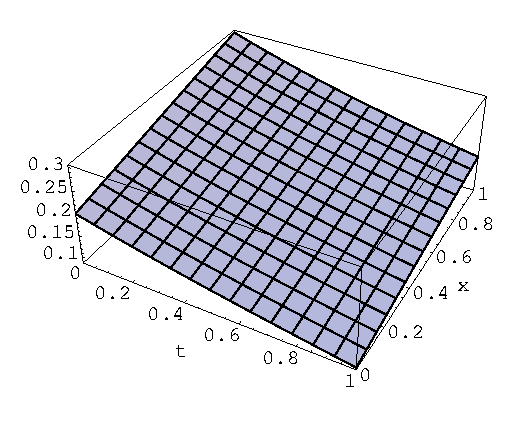
\includegraphics{senu_gr1.eps}}}\hspace{5pt}
\subfigure[A slightly shorter sub-caption.]{
\resizebox*{5cm}{!}{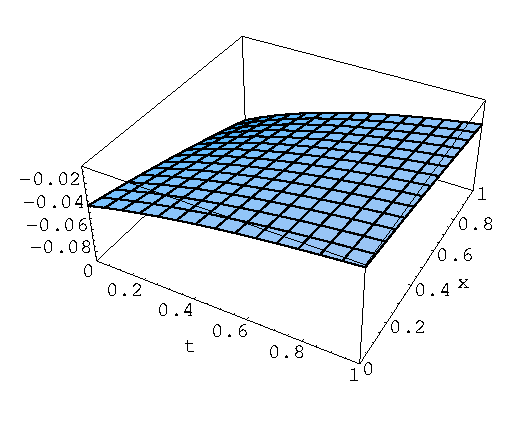
\includegraphics{senu_gr2.eps}}}
\caption{Example of a two-part figure with individual sub-captions
 showing that captions are flush left and justified if greater
 than one line of text, otherwise centred below the figure.}
\label{sample-figure}
\end{center}
\end{figure}
\end{verbatim}

\begin{figure}
\begin{center}
\subfigure[An example of an individual figure sub-caption.]{
\resizebox*{5cm}{!}{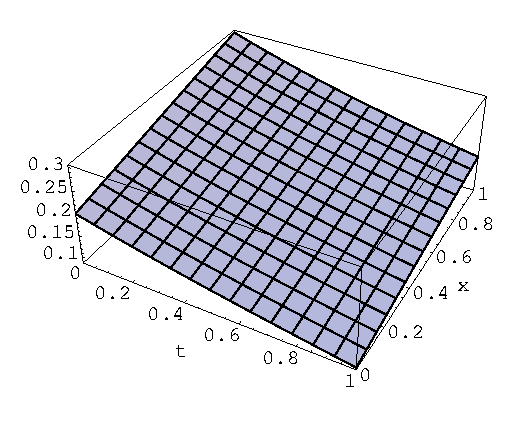
\includegraphics{senu_gr1.eps}}}\hspace{5pt}
\subfigure[A slightly shorter sub-caption.]{
\resizebox*{5cm}{!}{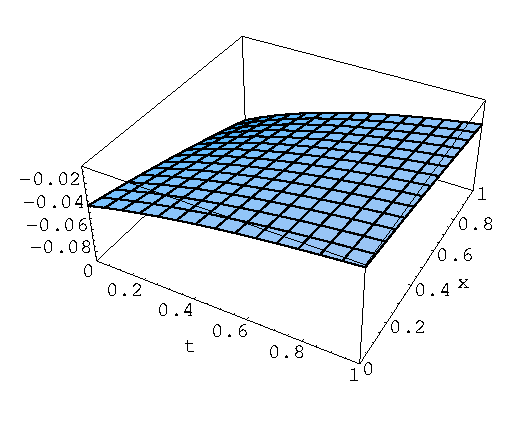
\includegraphics{senu_gr2.eps}}}
\caption{Example of a two-part figure with individual sub-captions
 showing that captions are flush left and justified if greater
 than one line of text, otherwise centred below the figure.}
\label{sample-figure}
\end{center}
\end{figure}

The \verb"\subfigure{}" and \verb"\includegraphics{}" commands require subfigure.sty and graphicx.sty.
The former is called in the preamble of the \texttt{gCOVguide.tex} file (in order to allow your choice of an alternative package if preferred)
and the latter by the \texttt{gCOV2e} class file; both are included with the \LaTeX\ style guide package for this journal for convenience.
Please supply any additional figure macros you use with your article in the preamble of your .tex file before \verb"\begin{document}".

To ensure that figures are correctly numbered automatically, the \verb"\label{}" command should be inserted just
after the \verb"\caption{}" command, or in its argument.

The \texttt{epstopdf} package can be used to incorporate Encapsulated PostScript (.eps) illustrations when using PDF\LaTeX, etc.
Please provide the original .eps source files rather than the generated PDF images of those illustrations for production purposes.


\subsection{Tables}

The \textit{gCOV} class file will cope with most positioning of your tables and you should not normally need to use the optional
placement specifiers of the \texttt{table} environment.

The \texttt{tabular} environment can be used as illustrated here to produce tables with appropriately spaced single thick and thin
horizontal rules, which are allowed, if desired. Thick rules should be used at the head and foot only, and thin rules elsewhere as appropriate.
Commands to redefine quantities such as \verb"\arraystretch" should be omitted.

The table caption appears above the body of the table in \textit{gCOV} style, therefore the \verb"\tbl" command should be used before the body of the table.
For example, Table~\ref{sample-table} is produced using the following commands. Note that \verb"\rm" will produce a roman character in math mode.
There are also \verb"\bf" and \verb"\it", which produce bold face and text italic in math mode.

\begin{table}
\tbl{Example of a table showing that its caption is as wide as the
 table itself and justified.}
{\begin{tabular}[l]{@{}lcccccc}\toprule
  Class$^{\rm a}$ & $\gamma _1$ & $\gamma _2$$^{\rm b}$
         & $\langle \gamma \rangle$
         & $G$ & $|{\bm f}|$ & $\theta _{c}$ \\
\colrule
  BL Lacs & 5 & 36 & 7 & $-4.0$ & $1.0\times 10^{-2}$ & 10$^\circ$ \\
  FSRQs & 5 & 40 & 11 & $-2.3$ & $0.5\times 10^{-2}$ & 14$^\circ$ \\
\botrule
\end{tabular}}
\tabnote{$^{\rm a}$This footnote shows what footnote symbols to use.}
\tabnote{$^{\rm b}$This footnote shows the text turning over when a long footnote is added.}
\label{sample-table}
\end{table}

\begin{verbatim}
\begin{table}
\tbl{Example of a table showing that its caption is as wide as the
 table itself and justified.}
{\begin{tabular}[l]{@{}lcccccc}\toprule
  Class$^{\rm a}$ & $\gamma _1$ & $\gamma _2$$^{\rm b}$
         & $\langle \gamma \rangle$
         & $G$ & $|{\bm f}|$ & $\theta _{c}$ \\
\colrule
  BL Lacs & 5 & 36 & 7 & $-4.0$ & $1.0\times 10^{-2}$ & 10$^\circ$ \\
  FSRQs & 5 & 40 & 11 & $-2.3$ & $0.5\times 10^{-2}$ & 14$^\circ$ \\
\botrule
\end{tabular}}
\tabnote{$^{\rm a}$This footnote shows what footnote symbols to use.}
\tabnote{$^{\rm b}$This footnote shows the text turning over when a
 long footnote is added.}
\label{sample-table}
\end{table}
\end{verbatim}

To ensure that tables are correctly numbered automatically, the \verb"\label{}" command should be inserted just before \verb"\end{table}".

Tables produced using the \texttt{booktabs} package of macros for typesetting tables are also compatible with the \textit{gCOV} class file.


\subsection{Landscape pages}\label{landscape}

If a table or illustration is too wide to fit the measure it will need to be turned, along with its caption, through 90$^{\circ}$ anticlockwise.
Landscape illustrations and/or tables can be produced using the \verb"rotating" package, which is called by the \textit{gCOV} class file.
The following commands (for example) can be used to produce such pages.
\begin{verbatim}
\setcounter{figure}{0}
\begin{sidewaysfigure}
\centerline{\epsfbox{figname.eps}}
\caption{Example landscape figure caption.}
\label{landfig}
\end{sidewaysfigure}
\end{verbatim}

\begin{verbatim}
\setcounter{table}{0}
\begin{sidewaystable}
 \tbl{Example landscape table caption.}
  {\begin{tabular}{@{}llllcll}
    .
    .
    .
  \end{tabular}}\label{landtab}
\end{sidewaystable}
\end{verbatim}
Before any such float environment, use the \verb"\setcounter" command as above to fix the numbering of the caption.
Subsequent captions will then be automatically renumbered accordingly.
The \verb"\epsfbox{}" command requires epsfig.sty, which is called by the \texttt{gCOV2e} class file and included with the \LaTeX\ style guide package for this journal for convenience.


\subsection{Theorem-like environments}

A predefined \verb"proof" environment is provided by the \texttt{amsthm} package (which is called by the \textit{gCOV} class file), as follows:

\begin{proof}
More recent algorithms for solving the semidefinite programming
relaxation are particularly efficient, because they explore the
structure of the MAX-CUT problem.
\end{proof}
\noindent This was produced by simply typing:
\begin{verbatim}
\begin{proof}
More recent algorithms for solving the semidefinite programming
relaxation are particularly efficient, because they explore the
structure of the MAX-CUT problem.
\end{proof}
\end{verbatim}
Other theorem-like environments (theorem, lemma, corollary, etc.) need to be defined as required, e.g. using \verb"\newtheorem{theorem}{Theorem}[section]"
in the preamble of your .tex file before \verb"\begin{document}". Theorem-like structures in \textit{gCOV} are generally numbered as per the following examples:

\begin{theorem}
More recent algorithms for solving the semidefinite programming
relaxation are particularly efficient, because they explore the
structure of the MAX-CUT problem.
\end{theorem}
\begin{lemma}
More recent algorithms for solving the semidefinite programming
relaxation are particularly efficient, because they explore the
structure of the MAX-CUT problem.
\end{lemma}
\begin{corollary}
More recent algorithms for solving the semidefinite programming
relaxation are particularly efficient, because they explore the
structure of the MAX-CUT problem.
\end{corollary}
\begin{proposition}
More recent algorithms for solving the semidefinite programming
relaxation are particularly efficient, because they explore the
structure of the MAX-CUT problem.
\end{proposition}
\begin{definition}
More recent algorithms for solving the semidefinite programming
relaxation are particularly efficient, because they explore the
structure of the MAX-CUT problem.
\end{definition}
\begin{remark}
More recent algorithms for solving the semidefinite programming
relaxation are particularly efficient, because they explore the
structure of the MAX-CUT problem.
\end{remark}

\noindent These were defined as shown in detail in the preamble of the \texttt{gCOVguide.tex} file, and produced by typing, for example:
\begin{verbatim}
\begin{theorem}
More recent algorithms for solving the semidefinite programming
relaxation are particularly efficient, because they explore the
structure of the MAX-CUT problem.
\end{theorem}
\end{verbatim}
The format of the text in these environments may be changed if necessary to match the style of the journal by the typesetter during preparation of your proofs.


\subsection{Typesetting mathematics}\label{maths}

\subsubsection{Displayed mathematics}

The \textit{gCOV} class file will set displayed mathematics centred on the measure without equation numbers if the \LaTeX\ standard commands open (\verb"\[") and close (\verb"\]") square brackets are used as
delimiters. The equation
\[
  \sum_{i=1}^p \lambda_i = {\rm trace}({\textrm{\bf S}})\qquad
  i\in {\mathbb R}
\]
\normalfont was typeset using the commands
\begin{verbatim}
\[
  \sum_{i=1}^p \lambda_i = {\rm trace}({\textrm{\bf S}})\qquad
  i\in {\mathbb R}
\]
\end{verbatim}

For those of your equations that you wish to be automatically numbered sequentially throughout the text,
use the \texttt{equation} environment, e.g.
\begin{equation}
  \sum_{i=1}^p \lambda_i = {\rm trace}({\textrm{\bf S}})\qquad
  i\in {\mathbb R}
\end{equation}
was typeset using the commands
\begin{verbatim}
\begin{equation}
  \sum_{i=1}^p \lambda_i = {\rm trace}({\textrm{\bf S}})quad
  i\in {\mathbb R}
\end{equation}
\end{verbatim}

Part numbers for sets of equations may be generated using the \texttt{subequations} environment, e.g.
\begin{subequations} \label{subeqnexample}
\begin{equation}
        \varepsilon \rho w_{tt}(s,t)
        =
        N[w_{s}(s,t),w_{st}(s,t)]_{s},
        \label{subeqnpart}
\end{equation}
\begin{equation}
        w_{tt}(1,t)+N[w_{s}(1,t),w_{st}(1,t)] = 0,
\end{equation}
\end{subequations}
which was generated using the commands
\begin{verbatim}
\begin{subequations} \label{subeqnexample}
\begin{equation}
        \varepsilon \rho w_{tt}(s,t)
        =
        N[w_{s}(s,t),w_{st}(s,t)]_{s},
        \label{subeqnpart}
\end{equation}
\begin{equation}
        w_{tt}(1,t)+N[w_{s}(1,t),w_{st}(1,t)] = 0,
\end{equation}
\end{subequations}
\end{verbatim}
This is made possible by the \texttt{subeqn} package, which is called
by the class file. If you put the \verb"\label{}" just after the
\verb"\begin{subequations}" line, references will be to the
collection of equations, `(\ref{subeqnexample})' in the example
above. Or, like the example code above, you can reference each
equation individually -- e.g. `(\ref{subeqnpart})'.

Displayed mathematics should be given end-of-line punctuation appropriate to the running text sentence of which it forms a part, if required.

\subsubsection{Bold math italic symbols}

To get bold math italic you can use \verb"\bm", which works for all sizes, e.g.
\begin{verbatim}
\sffamily
\begin{equation}
  {\rm d}({\bm s_{t_{\bm u}}) = \langle{\bm\alpha({\sf{\textbf L}})}
  [RM({\bm X}_y + {\bm s}_t) - RM({\bm x}_y)]^2 \rangle
\end{equation}
\normalfont
\end{verbatim}
produces\sffamily
\begin{equation}
  {\rm d}({\bm s_{t_{\bm u}}}) = \langle {\bm\alpha({\sf{\textbf L}})}[RM({\bm X}_y
  + {\bm s}_t) - RM({\bm x}_y)]^2 \rangle
\end{equation}\normalfont
Note that subscript, superscript, subscript to subscript, etc.
sizes will take care of themselves and are italic, not bold,
unless coded individually. \verb"\bm" produces the same effect as
\verb"\boldmath". \verb"\sffamily"...\verb"\normalfont" allows
upright sans serif fonts to be created in math mode by using the
control sequence `\verb"\sf"'.

\subsubsection{Bold Greek}\label{boldgreek}

Bold lowercase as well as uppercase Greek characters can be
obtained by \verb"{\bm \gamma}", which gives ${\bm \gamma}$, and
\verb"{\bm \Gamma}", which gives ${\bm \Gamma}$.

\subsubsection{Upright lowercase Greek characters and the upright partial derivative sign}\label{upgreek}

Upright lowercase Greek characters can be obtained with the \textit{gCOV} class file by inserting the letter `u' in the control
code for the character, e.g. \verb"\umu" and \verb"\upi" produce $\umu$ (used, for example, in the symbol for the
unit microns -- $\umu{\rm m}$) and $\upi$ (the ratio of the circumference to the diameter of a circle). Similarly,
the control code for the upright partial derivative $\upartial$ is \verb"\upartial".


\subsection{Acknowledgements}

An unnumbered section, e.g.\ \verb"\section*{Acknowledgement(s)}", should be used for thanks, etc.
and included \emph{in the non-anonymous version} before any Notes or References section.


\subsection{Disclosure}

An unnumbered section, e.g.\ \verb"\section*{Disclosure}", should be used to state any potential conflict of interest
and included \emph{in the non-anonymous version} before the References section, after any Acknowledgements and before any Funding statement.


\subsection{Funding}

An unnumbered section, e.g.\ \verb"\section*{Funding}", should be used for grant details, etc.
and included \emph{in the non-anonymous version} before any Notes or References section.


\subsection{Notes}

An unnumbered `Notes' section may be placed before the References section (if using the \verb"endnotes" package, use the command \verb"\theendnotes" where the notes are to appear instead of creating a \verb"\section").


\subsection{Supplemental material}

Supplemental material should be referenced within your article where appropriate. An unnumbered section, e.g. \verb"\section*{Supplemental material}", detailing the supplemental material available should be placed immediately before the list of references, and should include a brief description of each supplemental file.


\subsection{References}\label{refs}

\subsubsection{References cited in the text}

References should be cited in accordance with US National Library of Medicine (NLM) style (please refer to the style guide in the journal's Instructions for Authors for details). References are cited in the text by a number in square brackets (e.g. [1], [2,4,10], [11--15], not [11]--[15]), in the order in which they first appear.

Each bibliographical entry has a key, which is assigned by the author and used to refer to that entry in the text. In this document, the key \verb"neu83" in the citation form
\verb"\cite{neu83}" produces `\cite{neu83}', and the keys \verb"ed84" and \verb"aiex00" in the citation form
\verb"\cite{ed84,aiex00}" produce `\cite{ed84,aiex00}'. The citation for a range of bibliographic entries (e.g.
`\cite{Eri1984,glov00,hk97,glov86,Agu95,Holl04,Shak78,Mil93}') will automatically be produced by
\verb"\cite{Eri1984,glov00,hk97,glov86,Agu95,Holl04,Shak78,Mil93}". Optional notes may be included at the end of a citation by the use of square brackets, e.g. \verb"\cite[see][p.73-–77]{cwm73}" produces `\cite[see][p.73--77]{cwm73}'.

\subsubsection{The list of references}

References should be listed at the end of the main text in the order in which they are first cited in the text. The following list shows some references prepared in the style of the journal.

\begin{thebibliography}{99}

\bibitem{neu83}%1
Neumann M. Parallel GRASP with path-relinking for job shop scheduling. Mol
  Phys. 1983;50:841--843.

\bibitem{ed84}%2
Edwards DMF, McDonald IR. Positive bases in numerical optimization. Comput
  Optim Appl. 1984;21:169--175.

\bibitem{aiex00}%3
Aiex RM, Pierce IF, Donizetti G, von~Weber CM, Bizet G, Bach CPE, Strauss
  R, van~Beethoven L, Mozart WA, Dukas P. Computing tools for modelling
  orchestral performance. Cambridge (UK): University of Cambridge; 2000.
  Report No.: DAMTP 2000/NA10.

\bibitem{Eri1984}%4
Ericsson KA, Simon HA. Protocol analysis: verbal reports as data. Cambridge
  (MA): MIT Press; 1984.

\bibitem{glov00}%5
Glover F. Multi-start and strategic oscillation methods -- principles to exploit
  adaptive memory. In: Laguna M, Gonz\'{a}les-Velarde JL, editors. Computing
  tools for modeling, optimization and simulation: interfaces in computer
  science and operations research. 2nd ed. Vol.~2. Boston (MA): Kluwer Academic;
  2000. p. 1--24.

\bibitem{hk97}%6
Kern H. The resurgent Japanese economy and a Japan--United States free
  trade agreement. In: Lambert C, Holst G, editors. 4th International
  Conference on the Restructuring of the Economic and Political System in Japan
  and Europe; 1996 May 21--25; Milan, Italy. Singapore: World Scientific;
  1997. p. 147--156.

\bibitem{glov86}%7
Glover F. Hilbert modular forms and the Galois representations associated to
  Hilbert--Blumenthal abelian varieties [dissertation]. Cambridge (MA): Harvard
  University; 1986.

\bibitem{Agu95}%8
Agutter AJ. The linguistic significance of current British slang [unpublished
  doctoral dissertation]. Edinburgh (UK): Edinburgh University; 1995.

\bibitem{Holl04}%9
Holland M. Guide to citing internet sources. 2004~[cited~2012 Nov 4].
  Available from: http://www.bournemouth.ac.uk/library/using/guide\_to\_citing\_internet\_sourc.html.

\bibitem{Shak78}%10
Shakelford RT. Surgery of the alimentary tract. Philadelphia (PA): W.B.
Saunders; 1978. Chapter 2, Esophagoscopy; p. 29--40.

\bibitem{Mil93}%11
Miller ME. The interactive tester (version 4.0) [computer software].
  Westminster (CA): Psytek Services; 1993.

\bibitem{cwm73}%12
Misner CW. Efficient algorithms for layer assignment problems. In: Gottlob I,
  editor. Gravitation in a collapsing Universe. 2nd ed. San Francisco (CA):
  Freeman; 1973. p. 63--83. (Einstein's legacy; vol.~5).

\end{thebibliography}
\bigskip
\noindent This was produced by typing:
\begin{verbatim}
\begin{thebibliography}{99}

\bibitem{neu83}%1
Neumann M. Parallel GRASP with path-relinking for job shop
 scheduling. Mol Phys. 1983;50:841--843.

\bibitem{ed84}%2
Edwards DMF, McDonald IR. Positive bases in numerical optimization.
 Comput Optim Appl. 1984;21:169--175.

\bibitem{aiex00}%3
Aiex RM, Pierce IF, Donizetti G, von~Weber CM, Bizet G, Bach CPE,
 Strauss R, van~Beethoven L, Mozart WA, Dukas P. Computing tools
 for modelling orchestral performance. Cambridge (UK): University
 of Cambridge; 2000. Report No.: DAMTP 2000/NA10.

\bibitem{Eri1984}%4
Ericsson KA, Simon HA. Protocol analysis: verbal reports as data.
 Cambridge (MA): MIT Press; 1984.

\bibitem{glov00}%5
Glover F. Multi-start and strategic oscillation methods -- principles
 to exploit adaptive memory. In: Laguna M, Gonz\'{a}les-Velarde JL,
 editors. Computing tools for modeling, optimization and simulation:
 interfaces in computer science and operations research. 2nd ed.
 Vol.~2. Boston (MA): Kluwer Academic; 2000. p. 1--24.

\bibitem{hk97}%6
Kern H. The resurgent Japanese economy and a Japan--United States
 free trade agreement. In: Lambert C, Holst G, editors. 4th
 International Conference on the Restructuring of the Economic
 and Political System in Japan and Europe; 1996 May 21--25;
 Milan, Italy. Singapore: World Scientific; 1997. p. 147--156.

\bibitem{glov86}%7
Glover F. Hilbert modular forms and the Galois representations
 associated to Hilbert--Blumenthal abelian varieties [dissertation].
 Cambridge (MA): Harvard University; 1986.

\bibitem{Agu95}%8
Agutter AJ. The linguistic significance of current British slang
 [unpublished doctoral dissertation]. Edinburgh (UK): Edinburgh
 University; 1995.

\bibitem{Holl04}%9
Holland M. Guide to citing internet sources. 2004 [cited~2012 Nov 4].
 Available from:
 http://www.bournemouth.ac.uk/library/using/guide\_to\_citing\_internet\_sourc.html.

\bibitem{Shak78}%10
Shakelford RT. Surgery of the alimentary tract. Philadelphia (PA):
 W.B. Saunders; 1978. Chapter 2, Esophagoscopy; p. 29--40.

\bibitem{Mil93}%11
Miller ME. The interactive tester (version 4.0) [computer software].
 Westminster (CA): Psytek Services; 1993.

\bibitem{cwm73}%12
Misner CW. Efficient algorithms for layer assignment problems. In:
 Gottlob I, editor. Gravitation in a collapsing Universe. 2nd ed.
 San Francisco (CA): Freeman; 1973. p. 63--83. (Einstein's legacy;
 vol.~5).

\end{thebibliography}
\end{verbatim}
\bigskip
\noindent Each entry takes the form:
\begin{verbatim}
\bibitem{key} Bibliography entry
\end{verbatim}
where `\texttt{key}' is the tag that is to be used as an argument for the \verb"\cite{}" commands in the text of the article and \texttt{Bibliography entry} is the material that is to appear in the list of references, suitably formatted.

Instead of typing the bibliography by hand, you may prefer to create the list of references using a \textsc{Bib}\TeX\ database. Include the lines
\begin{verbatim}
\bibliographystyle{gCOV}
\bibliography{gCOVguide}
\end{verbatim}
where the list of references should appear, where \texttt{gCOV.bst} is the name of the \textsc{Bib}\TeX\ style file for this journal and \texttt{gCOVguide.bib} is the database of bibliographic details for the references section included with the \textit{gCOV} \LaTeX\ style guide package (to be replaced with the name of your own \textsc{Bib}\TeX\ database). The \LaTeX\ source file of your paper will extract from your .bib file only those references that are cited in that paper and list them in the References section of it.

Please include a copy of your .bib file and/or the final generated .bbl file among your source files if your .tex file does not contain a reference list in a \texttt{thebibliography} environment.


\subsection{Appendices}\label{appendices}

Any appendices should be placed after the list of references, beginning with the
command \verb"\appendices" followed by the command \verb"\section"
for each appendix title, e.g.
\begin{verbatim}
\appendices
\section{This is the title of the first appendix}
\section{This is the title of the second appendix}
\end{verbatim}

\noindent produces:\medskip

\noindent\textbf{Appendix A. This is the title of the first appendix}\medskip

\noindent\textbf{Appendix B. This is the title of the second appendix}\medskip

\noindent Subsections, equations, figures, tables, etc. within
appendices will then be automatically numbered as appropriate.


\section{Example of a section heading including {\fontencoding{T1}\scshape{small caps}},
   \textit{italic}, and bold Greek such as ${\bm\kappa}$}\label{headings}

The following code shows how to achieve this section heading:
\begin{verbatim}
\section{Example of a section heading including
 {\fontencoding{T1}\scshape{small caps}}, \textit{italic},
 and bold Greek such as ${\bm\kappa}$}\label{headings}
\end{verbatim}


\section{\textit{gCOV} journal style}

The notes given here relate to common style errors found in manuscripts, but are \emph{not}
intended to be exhaustive.


\subsection{Hyphens, en rules, em rules and minus signs}\label{dashes}

\begin{enumerate}
\item[(i)] Hyphens (one dash in \TeX/\LaTeX). \textit{gCOV} uses hyphens for compound adjectives (e.g.\ low-density gas, least-squares fit,
two-component model) but not for complex units or ranges, which could become cumbersome (e.g.\ 15~km~s$^{-1}$
feature, 100--200~$\umu$m observations).

\item[(ii)] en rules (two dashes in \TeX/\LaTeX). These are used (a) to denote a range (e.g.\ 1.6--2.2~$\umu$m);
(b) to denote the joining of two words of equal standing (e.g.\ Kolmogorov--Smirnov test, Herbig--Haro object);
(c) with spaces, as an alternative to parentheses (e.g.\ `the results -- assuming no temperature gradient -- are indicative of \ldots').

\item[(iii)] The em rule (three dashes in \TeX/\LaTeX) has no specified use in \textit{gCOV}.

\item[(iv)] The minus sign is produced automatically in math mode by the use of a single dash, e.g.
\begin{equation}
y_{i} \in \{-1, 1 \} \quad \forall i \in V,
\end{equation}
\noindent where $|-V|=A^2+B^2.$\medskip

\noindent is produced by
\begin{verbatim}
\begin{equation}
y_{i} \in \{-1, 1 \} \quad \forall i \in V,
\end{equation}
\noindent where $|-V|=A^2+B^2.$
\end{verbatim}

\end{enumerate}


\subsection{References}

It is important to use the correct reference style, details of which can be found in Section~\ref{refs}.


\subsection{Maths fonts}

Scalar variables should be mediumface italic (e.g.\ $s$ for speed);
vectors should be bold italic (e.g.\ $\bm v$ for velocity);
matrices should be bold roman (upright) (e.g.\ $\bf A$), and
tensors should be bold upright sans serif (e.g.\ {\sffamily{\textbf L}}).
Differential d, partial differential $\upartial$, complex i,
exponential e, superscript T for `transpose', sin, cos, tan, log, etc.,
should all be roman. Openface, or `blackboard', fonts can be used,
for example, for the integers $\mathbb Z$ and the reals $\mathbb R$.
Sub/superscripts that are physical variables should be italic,
while those that are labels should be roman (e.g.\ $C_p$, $T_{\rm eff}$).


\section{Troubleshooting}

Authors may from time to time encounter problems with the preparation
of a paper using \LaTeX\/. The appropriate action to take will depend
on the nature of the problem -- the following is intended as a guide.

\begin{enumerate}
\item[(i)] If the problem is with \LaTeX\ itself, rather than with the
actual macros, please refer to an appropriate handbook for
initial advice. If the solution cannot be found, or if you
suspect that the problem lies with the macros, then please contact
Taylor \& Francis for assistance (\texttt{latex.helpdesk@tandf.co.uk}).

\item[(ii)] Problems with page make-up (e.g.\ large spaces between paragraphs,
above headings, or below figures; figures/tables appearing out of order):
please do not attempt to remedy these using `hard' page make-up
commands -- the typesetter will deal with such problems. (You may, if you
wish, draw attention to particular problems when submitting the final version
of your paper.)

\item[(iii)] If a required font is not available at your site, allow \TeX\
to substitute the font and specify which font you require in a covering letter
accompanying your file(s).
\end{enumerate}


\section{Fixes for coding problems}

This guide has been designed to minimize the need for user-defined macros to create special symbols. Authors
are urged, wherever possible, to use the following coding rather than to create their own. This will minimize
the danger of author-defined macros being accidentally `overridden' when the paper is typeset (see
Section~\ref{maths}, `Typesetting mathematics'). In cases where it is essential to create your own macros,
these should be displayed in the preamble of your \texttt{.tex} file before \verb"\begin{document}".

\begin{enumerate}
\item[(i)] Fonts in section headings and paper titles. The following are examples
of styles that sometimes prove difficult to code.


\subsection*{Paper titles:}

\hsize380pt\bf{\noindent Generalized Flory theory at ${\bm\delta >
{\bf 50}^\circ}$}\\

    \noindent\normalfont is produced by
\begin{verbatim}
\title{Generalized Flory theory at
        ${\bm\delta > {\bfseries 50}^\circ}$}
\end{verbatim}
\bigskip

{\bf{\noindent Ion--ion correlations in H\,{\sc ii} regions}}\\

\noindent\normalfont is produced by
\begin{verbatim}
\title{Ion--ion correlations in H\,{\sc ii} regions}
\end{verbatim}


\stepcounter{enumi}

\item[(ii)] en rules, em rules, hyphens and minus signs (see Section~\ref{dashes} for
correct usage). To create the correct symbols in the sentence
\begin{quote}
The high-resolution observations were made along a line at an
angle of $-15^\circ$ (East from North) from the axis of the
jet -- which runs North--South
\end{quote}
you would use the following code:
\begin{verbatim}
The high-resolution observations were made along a line at an
angle of $-15^\circ$ (East from North) from the axis of the
jet -- which runs North--South
\end{verbatim}

\item[(iii)] Fonts in superscripts and subscripts. Subscripts and superscripts will automatically come out in the correct font
and size in a math environment (e.g. enclosed by `\verb"$"'
delimiters in running text or within \verb"\[...\]" or the
`\texttt{equation}' environment for displayed equations). You can create
the output ${\bm k_x}$ by typing \verb"${\bm k_x}$". If the
subscripts or superscripts need to be other than italic, they
should be coded individually -- see (vi) below.

\item[(iv)] Calligraphic letters ($\mathcal{UPPER\ CASE\ ONLY}$).
Normal calligraphic can be produced with \verb"\mathcal" as usual (in math mode).

\item[(v)] Automatic scaling of brackets. The codes \verb"\left" and
\verb"\right" should  be used to scale brackets automatically to
fit the equation being set. For example, to get
\[
   v = x \left( \frac{N+2}{N} \right)
\]
use the code
\begin{verbatim}
\[
   v = x \left( \frac{N+2}{N} \right)
\]
\end{verbatim}

\item[(vi)] Roman font in equations. It is often necessary to make some
symbols roman in an equation (e.g.\ units, non-variable subscripts).
For example, to get
\[
   \sigma \simeq (r/13~h^{-1}~{\rm Mpc})^{-0.9},
   \qquad \omega = \frac{N-N_{\rm s}}{N_{\rm R}}
\]
\noindent use the code
\begin{verbatim}
\[
   \sigma \simeq (r/13~h^{-1}
   ~{\rm Mpc})^{-0.9}, \qquad \omega
   =\frac{N-N_{{\rm s}}}{N_{{\rm R}}}
\]
\end{verbatim}
The \texttt{SIunits} package of macros for typesetting units is also compatible with the \texttt{gCOV2e} class file.
\end{enumerate}


\section{Obtaining the gCOV2e class file}\label{FTP}

\subsection{Via the Taylor \& Francis website}

This Guide for Authors and the \texttt{gCOV2e} class file may be obtained via the Instructions for Authors
on the Taylor \& Francis homepage for the journal.

Please note that the class file calls up the following open-source \LaTeX\ packages, which will, for convenience,
unpack with the downloaded Guide for Authors and class file: amsbsy.sty; amsfonts.sty; amsmath.sty; amssymb.sty; epsfig.sty; graphicx.sty; natbib.sty; rotating.sty.
The Guide for Authors calls for subfigure.sty, which is also supplied for convenience.


\subsection{Via e-mail}

This Guide for Authors, the class file and the associated open-source \LaTeX\ packages are also available by e-mail.
Requests should be addressed to \texttt{latex.helpdesk@tandf.co.uk} clearly stating for which journal you require the Guide for Authors and/or class file.

\end{document}
